\documentclass[bigtut]{quiz}\usepackage[]{graphicx}\usepackage[]{color}
%% maxwidth is the original width if it is less than linewidth
%% otherwise use linewidth (to make sure the graphics do not exceed the margin)
\makeatletter
\def\maxwidth{ %
  \ifdim\Gin@nat@width>\linewidth
    \linewidth
  \else
    \Gin@nat@width
  \fi
}
\makeatother

\definecolor{fgcolor}{rgb}{0.345, 0.345, 0.345}
\newcommand{\hlnum}[1]{\textcolor[rgb]{0.686,0.059,0.569}{#1}}%
\newcommand{\hlstr}[1]{\textcolor[rgb]{0.192,0.494,0.8}{#1}}%
\newcommand{\hlcom}[1]{\textcolor[rgb]{0.678,0.584,0.686}{\textit{#1}}}%
\newcommand{\hlopt}[1]{\textcolor[rgb]{0,0,0}{#1}}%
\newcommand{\hlstd}[1]{\textcolor[rgb]{0.345,0.345,0.345}{#1}}%
\newcommand{\hlkwa}[1]{\textcolor[rgb]{0.161,0.373,0.58}{\textbf{#1}}}%
\newcommand{\hlkwb}[1]{\textcolor[rgb]{0.69,0.353,0.396}{#1}}%
\newcommand{\hlkwc}[1]{\textcolor[rgb]{0.333,0.667,0.333}{#1}}%
\newcommand{\hlkwd}[1]{\textcolor[rgb]{0.737,0.353,0.396}{\textbf{#1}}}%

\usepackage{framed}
\makeatletter
\newenvironment{kframe}{%
 \def\at@end@of@kframe{}%
 \ifinner\ifhmode%
  \def\at@end@of@kframe{\end{minipage}}%
  \begin{minipage}{\columnwidth}%
 \fi\fi%
 \def\FrameCommand##1{\hskip\@totalleftmargin \hskip-\fboxsep
 \colorbox{shadecolor}{##1}\hskip-\fboxsep
     % There is no \\@totalrightmargin, so:
     \hskip-\linewidth \hskip-\@totalleftmargin \hskip\columnwidth}%
 \MakeFramed {\advance\hsize-\width
   \@totalleftmargin\z@ \linewidth\hsize
   \@setminipage}}%
 {\par\unskip\endMakeFramed%
 \at@end@of@kframe}
\makeatother

\definecolor{shadecolor}{rgb}{.97, .97, .97}
\definecolor{messagecolor}{rgb}{0, 0, 0}
\definecolor{warningcolor}{rgb}{1, 0, 1}
\definecolor{errorcolor}{rgb}{1, 0, 0}
\newenvironment{knitrout}{}{} % an empty environment to be redefined in TeX

\usepackage{alltt}
\unitcode{MATH1005}
        \unitname{Statistics}
        \semester{Semester2}
        \sheetnumber1
\IfFileExists{upquote.sty}{\usepackage{upquote}}{}
\begin{document}
\lettersfirst

\begin{tutorial}

{\bf Aim of Course}  \\
To develop foundational statistical literacy which can be transferred to any discipline: \\
how to understand data (Part1), how data arises from populations (Part2), and how to use data to test hypotheses and make inferences about the population (Part3).  \\ \\

{\small \begin{tabular}{|l|l|l|l|} \hline
{\bf Week} & {\bf Topic} \hspace{7cm} & {\bf Tute/Lab} \hspace{3cm} & {\bf Assessment} \hspace{.9cm} \\ \hline
  & {\bf 1. Exploratory Data Analysis} &    &  \\ \hline
1  & Topic1: Data and Graphical Summaries &  Intro Tute (Self Study)  &  \\
25-26/7 &  &   & \\
& & & \\ \hline
2 & Topic2: Numerical Summaries & Topic1 & \\
1-2/8  &   &  & \\ 
& & & \\ \hline
3 & Topic3: Bivariate Data & Topic2 & \\
8-9/8 & &   & \\
& & & \\ \hline
 & {\bf 2. Probability and Distribution Theory} & &   \\ \hline
4 & Topic4: Probability, RVs and Distributions &  Present Report1 & Report1 10\% \\
15-16/8 &   & Topic3 (Self Study) &  \\
& & & \\ \hline
5 & Topic5: Discrete Random Variables & Topic4 & Quiz1 5\%  \\
22-23/8 &  &   &  \\ 
& & & \\ \hline
6 & Topic6: Continuous Random Variables & Topic5 & \\
29-30/8 & & & \\ 
& & & \\ \hline
7 & Topic7: Combinations of Random Variables & Topic6 & \\
5-6/9 &  & & \\ 
& & & \\ \hline
 &  {\bf 3. Hypothesis Testing and Inference} &  & \\ \hline
8 &  Topic8: Hypothesis Testing  & Topic7 & Report2 5\% \\
12-13/9 &  &  &  \\ 
& & & \\ \hline
9 & Topic9: Tests for Proportion & Topic8  & Quiz2 5\%  \\
19-20/9 &  & &   \\ 
& & & \\ \hline
Break & & & \\ \hline
10 & Topic10: Tests for Means & Topic9 & \\
4/10 & & & \\ 
& & & \\ \hline
11 & Topic11: Test for Goodness of Fit    & Topic10 & \\
10-11/10 &    & & \\ 
& & & \\ \hline
12 & Topic12: Confidence Intervals  & Topic11 & Report3 5\% \\
17-18/10 &  & &  \\ 
& & & \\ \hline
13 & {\bf Revision} & Topic12 & Quiz3 5\% \\
24-25/10 & &  &   \\
& & & \\ \hline
\end{tabular} }



\newpage
{\bf Aim of Quizzes} \\
The Quizzes test basic statistical skills.   

{\small \begin{tabular}{|l|l|l|} \hline  
& & \\ 
 {\bf Quiz} \hspace{1cm} & {\bf Content} & {\bf Complete in Tute}  \\  [2ex]  \hline 
 & & \\ 
 {\bf Quiz1}  5\%  & Part 1: Exploratory Data Analysis &  Week5 \\
& &    \\ [2ex]  \hline 
& & \\ 
 {\bf Quiz2} 5\% & Part2: Probability and Distribution Theory &  Week9  \\
  & &  \\  [2ex]   \hline 
  & & \\  
{\bf Quiz3} 5\% & Part3: Hypothesis Testing and Inference (excluding Topic12) & Week13 \\
    & &   \\  [2ex]   \hline 
\end{tabular} }

\vspace{.5cm}
{\bf Quiz Instructions}
\begin{itemize}
\item Please bring your student card for identification.  \\ 
\item Quizzes are completed in the first 20 minutes of your designated tutorial class.  \\ 
\item Quizzes are completed online, using a link on the MATH1005 website.  \\ 
\item Each Quiz consist of 5 short questions requiring a numerical answer. \\
\item If the answer requires rounding, use up to 2dp.  \\
\item Use both hand working and R to doublecheck your calculations. \\ 
\item You may use a calculator and refer to the MATH1005 website but not have any hard copies of notes.  \\
\item To prepare, work through the practise questions and revise the relevant lectures and tutes. \\
\item The better mark principle automatically applies to the Quizzes. 
\end{itemize}

\newpage
{\bf Stats Reports} \\
The Stats Reports test statistical literacy and communication.   \\


{\small \begin{tabular}{|l|l|} \hline  
& \\ 
 {\bf Report Content} \hspace{1cm} & {\bf Due Date}  \\  [2ex]  \hline 
 & \\ 
{\bf Report1}  10\%   \hspace{.1cm} (Written Report 7\% + Verbal Report 3\%) & 15/8 11:59pm   \\
Investigate your own data and present a short talk  & $\bullet$ Submit PDF of Verbal Report through Turnitin      \\
to your tute class. & $\bullet$ Submit PDF of Written Report through Turnitin    \\
&     \\
Report1 is designed to give you experience with    & Week4: Present Verbal Report in Tute class.       \\ 
analysing data of your choice to illustrate the    &      \\ 
transfer of Statistics to any discipline. &   \\
&      \\  [2ex]  \hline 
 & \\  
 {\bf Report2} 5\% & 12/9 11:59pm: Submit PDF of  Report through Turnitin \\  
 Investigate the use of statistics in the media.  &    \\ [2ex]   \hline 
 & \\  
 {\bf Report3} 5\% & 17/10 11:59pm: Submit PDF of  Report through Turnitin \\ 
Investigate the use of statistics in a given research paper.  &    \\
  & \\   [2ex]   \hline 
\end{tabular} }

The better mark principle does not apply to the Reports. \\

\newpage
{\bf Report1 Instructions}
\begin{enumerate}
\item {\bf Collaboration} \\
Decide whether you are going to do the report alone or with someone in your tutorial class. Working as a pair helps to develop the skill of collaboration and usually improves the result. \\
\item {\bf Source Data} \\
Find a data set that you are interested in, ideally something related to your major or potential career.   Often a larger data set is more interesting, but dealing with small data sets is also an important skill. This can take many hours. It usually helps to search by the subject (eg Breast Cancer) and file type (eg .csv). \\
\item {\bf Import your Data into R} \\
See the Intro Tute for different methods. You must use R for your analysis. \\
\item {\bf Do Exploratory Data Analysis} \\
Using the techniques in Topics1-3, extract variables you are interested in, and explore your data. \\
\item {\bf Fill out Template (Written Report)} \\
Fill out the Template. Then attach your RCode (commands) and Data as pages 2 and 3. Save the whole file as a PDF. Name the file by the subject (eg BreastCancer.pdf). You will lose a mark for not using the Template and for going over the 1 page limit. \\

\noindent
Page1: Template (including relevant R output) \\
Page2: RCode (Commands) \\
Page3: Data \\

\item {\bf Produce a presentation (Verbal Report)} \\
Using your Written report as a guide, produce slides for presentation to your tutorial class. The content of the Verbal Report does not have to be the same as the Written Report - choose whatever is interesting for your class. Save the file as a PDF. Name the file by the subject (eg BreastCancerPresentation.pdf). \\
\item {\bf Submit both PDFs in Turnitin} \\
Submit your PDFs in Turnitin, using the file title as the Turnitin title. If you work as a pair, both students need to individually submit the same PDFs of the Verbal and Written Reports through Turnitin. No other form of documents (eg .docx, .pptx) will be marked. \\

\begin{center}
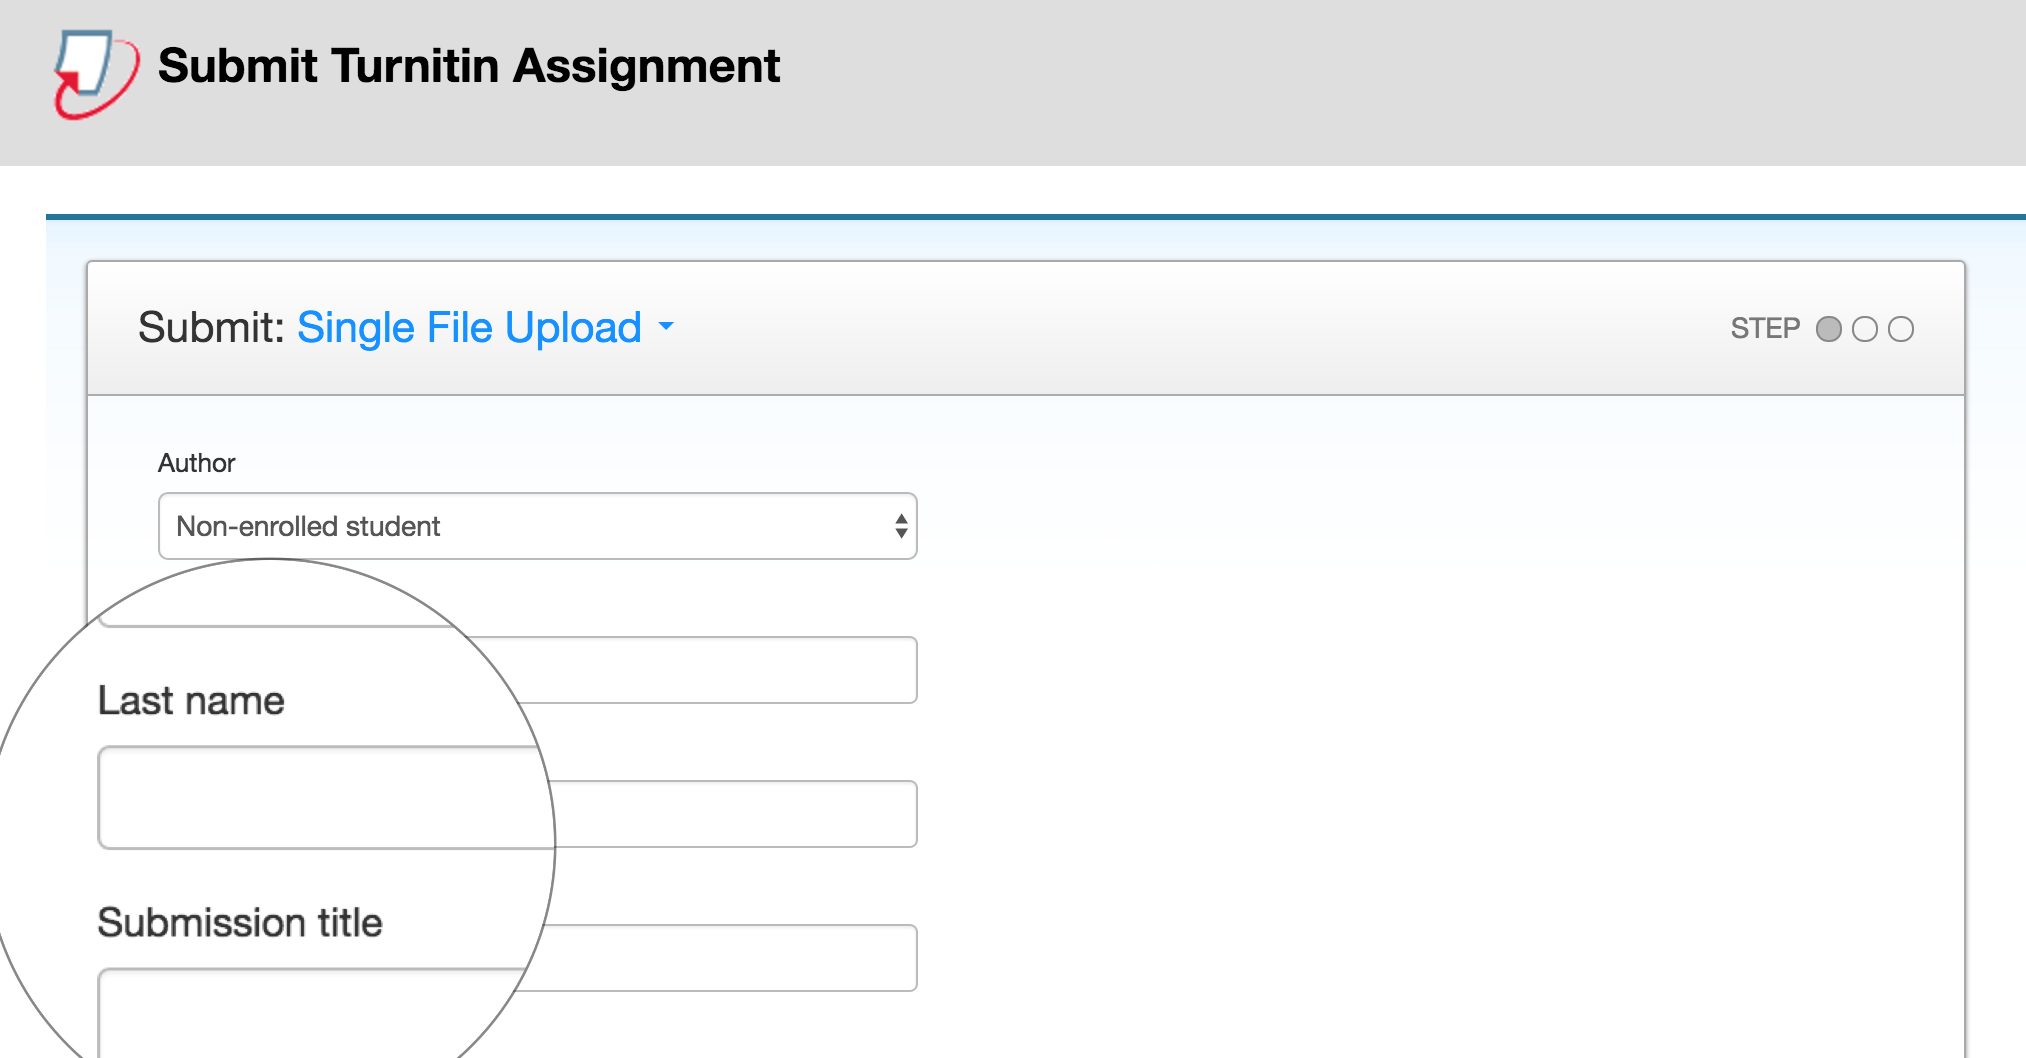
\includegraphics[height=4.5cm]{TurnitinSubmission.png}
\end{center}

\item {\bf Present in your class} \\
Your tutor will access your presentation file in Turnitin and put it on the big screen. You cannot bring your file on a USB. The Verbal Report is 2 mins long (with strict maximum of 2.5 mins). If the Verbal Report is presented as a pair, then both students must be part of the presentation (whether speaking or operating the slides).  \\

\noindent
{Marking Scheme for Verbal Report} \\
1 mark: Student(s) presents the Report with PDF. \\
1 mark: Student(s) explains an appropriate presentation of the data. \\
1 mark: Student(s) explain the motivation for the Report (eg impact or usefulness).
\end{enumerate}




\newpage
\fbox{ {\bf Stats Report 1 Written: Exploratory Data Analysis} } \\  {\tiny \bf  Submit 1 Page Template, plus the data and R Code attached, as PDF, through Turnitin.}

\begin{tabular}{|l|l|r|} \hline
{\bf Analysis} & {\bf Details} \hspace{11cm} & {\bf Mark} \\ \hline
Data & {\tiny What is your data? (Eg 2016 road fatalities in Australia)} & 1  \\
& & \\ 
Source & {\tiny Where did you find your data? (Eg Provide the url.) Attach your data.} &  \\ 
& & \\ 
Integrity &  {\tiny Give 1 reason that you trust its integrity.} &   \\ 
& & \\ \hline
Numerical  & {\tiny Present 2 summaries from R. What do they tell you about the data?}  & 3 \\ 
Summaries & & \\ 
& & \\ 
& & \\ 
& & \\
& & \\ 
& & \\ 
& & \\ 
& & \\ 
& & \\  
& & \\ 
& & \\ 
& & \\ 
& & \\
& & \\ \hline
Graphical & {\tiny Present an appropriate summary from R. What does it tell you about the data?}  & 2 \\ 
Summary & & \\ 
& & \\ 
& & \\ 
& & \\ 
& & \\ 
& & \\
& & \\ 
& & \\ 
& & \\ 
& & \\ 
& & \\ 
& & \\ 
& & \\ 
& & \\ 
& & \\ 
& & \\ 
& & \\ 
& & \\ 
& & \\ 
& & \\
& & \\ \hline
Usefulness & {\tiny Who might benefit from this analysis?} & 1 \\
& & \\
Research & {\tiny What is a question that could be investigated by further data analysis?} &  \\
& & \\
R Code & {\tiny Attach the R Code.} &  \\ 
& & \\ \hline
Total & &  \\ 
& & /7 \\ \hline
\end{tabular}


\newpage
{\bf Report2 Instructions}
\begin{enumerate}
\item {\bf Collaboration} \\
Decide whether you are going to do the report alone or with someone in your tutorial class. Working as a pair helps to develop the skill of collaboration and usually improves the result. \\
\item {\bf Source article in the media} \\
Find an article that you are interested in, which uses statistics. \\
\item {\bf Annotate article} \\
Critically read through the article annotating relevant parts.  \\
\item {\bf Fill out Template} \\
Fill out the Template. Then attach your annotated article as pages 2 and following. Save the whole file as a PDF. Name the file by the subject (eg BreastCancer.pdf). You will lose a mark for not using the Template and for going over the 1 page limit. \\
\item {\bf Submit PDF in Turnitin} \\
Submit your PDF in Turnitin, using the file title as the Turnitin title. If you work as a pair, both students need to individually submit the same PDF through Turnitin. No other form of document (eg .docx) will be marked. \\

\begin{center}
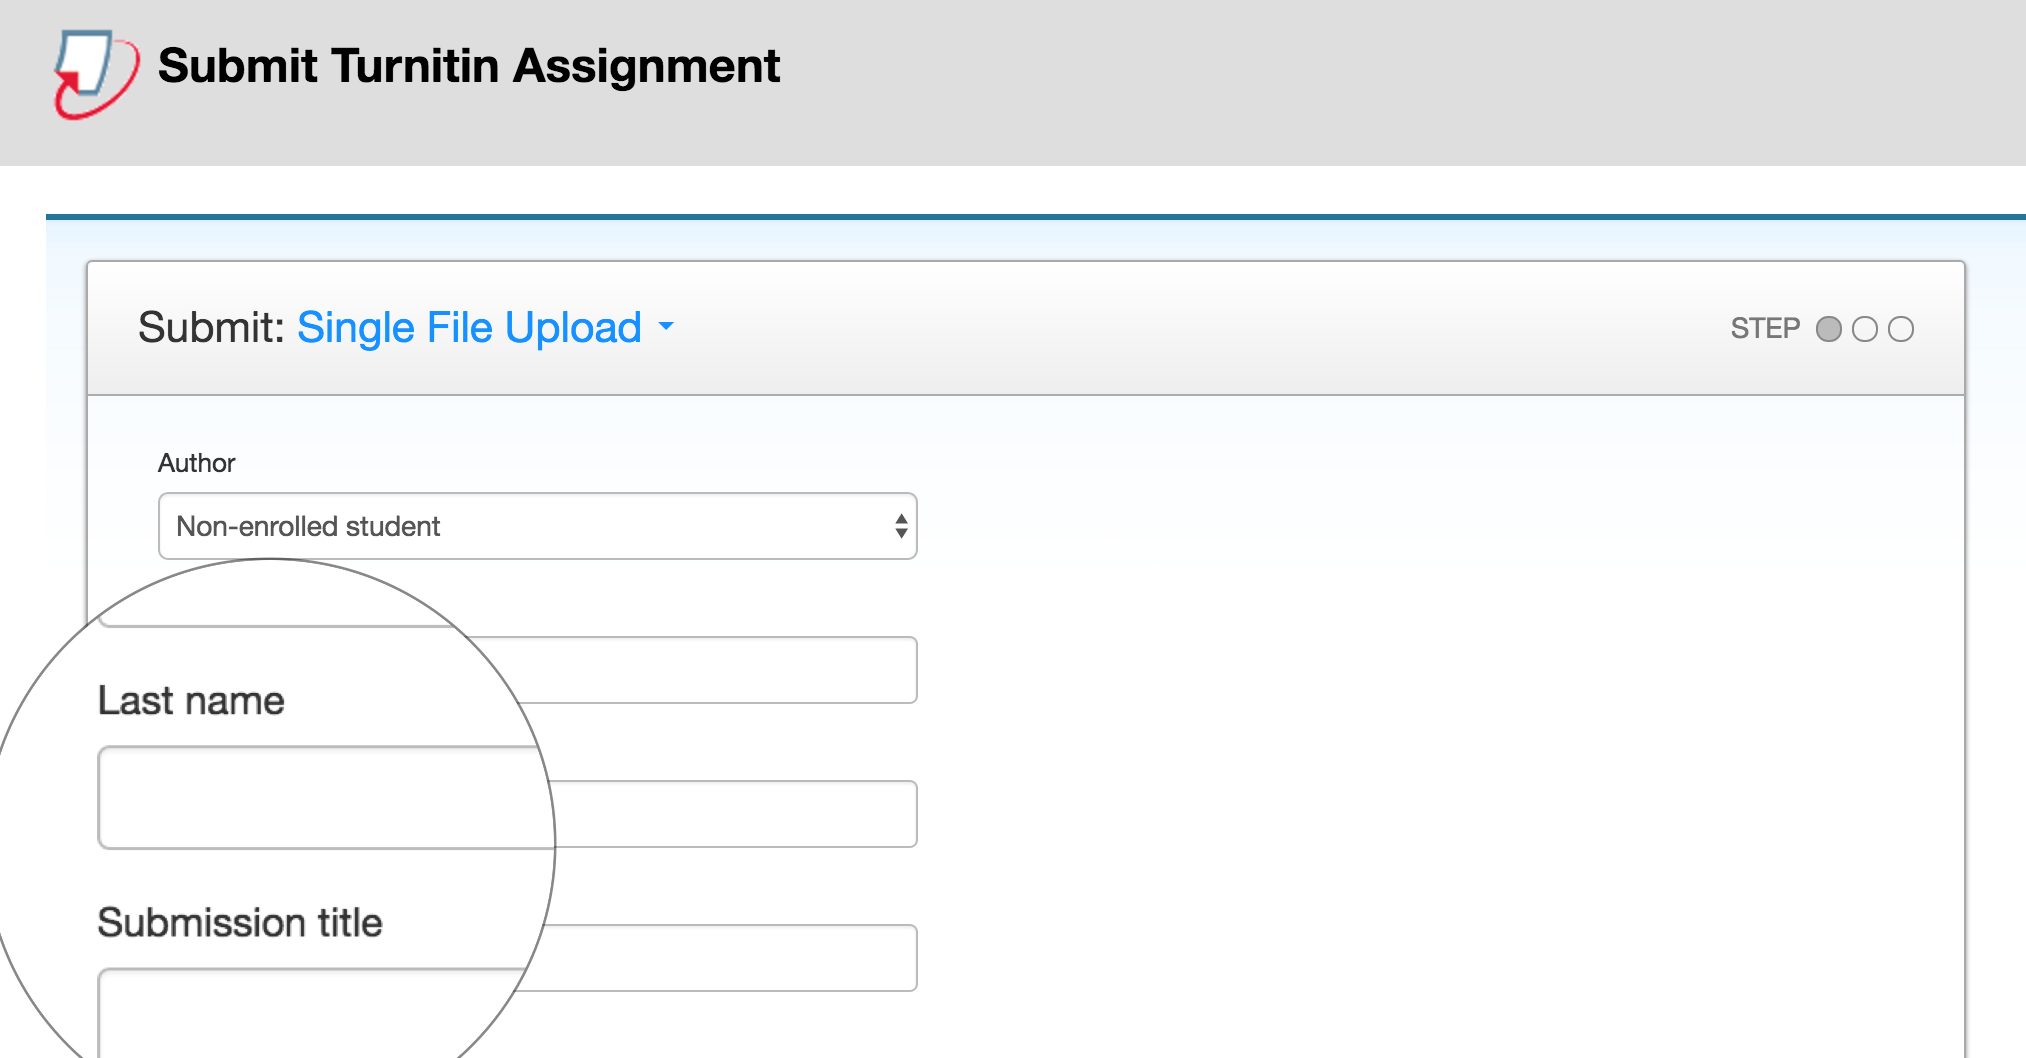
\includegraphics[height=4.5cm]{TurnitinSubmission.png}
\end{center}
\end{enumerate}


\newpage
\fbox{ {\bf Stats Report 2: Statistics in the Media} }  {\tiny \bf  Submit this 1 Page Template, plus the annotated Article attached.}

\begin{tabular}{|l|l|r|} \hline
{\bf Analysis} & {\bf Details} \hspace{11cm} & {\bf Mark} \\ \hline
Article & {\tiny What is the title and author of the article?} & 1  \\
& & \\ 
Source & {\tiny Where did you find the article? (Eg Provide the url.) Attach the article, with the relevant sections highlighted.} \hspace{.5cm} &  \\ 
& & \\ 
Integrity &  {\tiny Give 1 reason that you do or don't trust its integrity.} &   \\ 
& & \\ \hline
Summary & {\tiny How was statistics used in this article? For what purpose? Does the use of statistics support the author's conclusion?} & 3 \\
&  & \\ 
& & \\ 
& & \\ 
& & \\ 
& & \\  
& & \\ 
& & \\ 
& & \\  
& & \\
& & \\ 
& & \\ 
& & \\ 
& & \\ 
& & \\ 
& & \\ 
& & \\ 
& & \\ 
& & \\ 
& & \\ 
& & \\ 
& & \\ 
& & \\ 
& & \\ 
& & \\ 
& & \\ 
& & \\ 
& & \\ 
& & \\
& & \\ 
& & \\ 
& & \\ 
& & \\ 
& & \\ 
& & \\ 
& & \\ 
& & \\ 
& & \\ 
& & \\ 
& & \\ 
& & \\ 
& & \\\hline
Research & {\tiny What is a question that could be investigated by further data analysis?} & 1 \\
& & \\
& & \\
& & \\ \hline
Total & &  \\ 
& & /5 \\ \hline
\end{tabular}



\newpage
{\bf Report3 Instructions}
\begin{enumerate}
\item {\bf Collaboration} \\
Decide whether you are going to do the report alone or with someone in your tutorial class. Working as a pair helps to develop the skill of collaboration and usually improves the result. \\
\item {\bf Choose an article from those given, and read through carefully.} \\
 
\item {\bf Fill out Template} \\
Fill out the Template. Save the whole file as a PDF. Name the file by the subject (Sharks.pdf or Mobiles.pdf). You will lose a mark for not using the Template and for going over the 1 page limit. \\
\item {\bf Submit PDF in Turnitin} \\
Submit your PDF in Turnitin, using the file title as the Turnitin title. If you work as a pair, both students need to individually submit the same PDF through Turnitin. No other form of document (eg .docx) will be marked. \\

\begin{center}
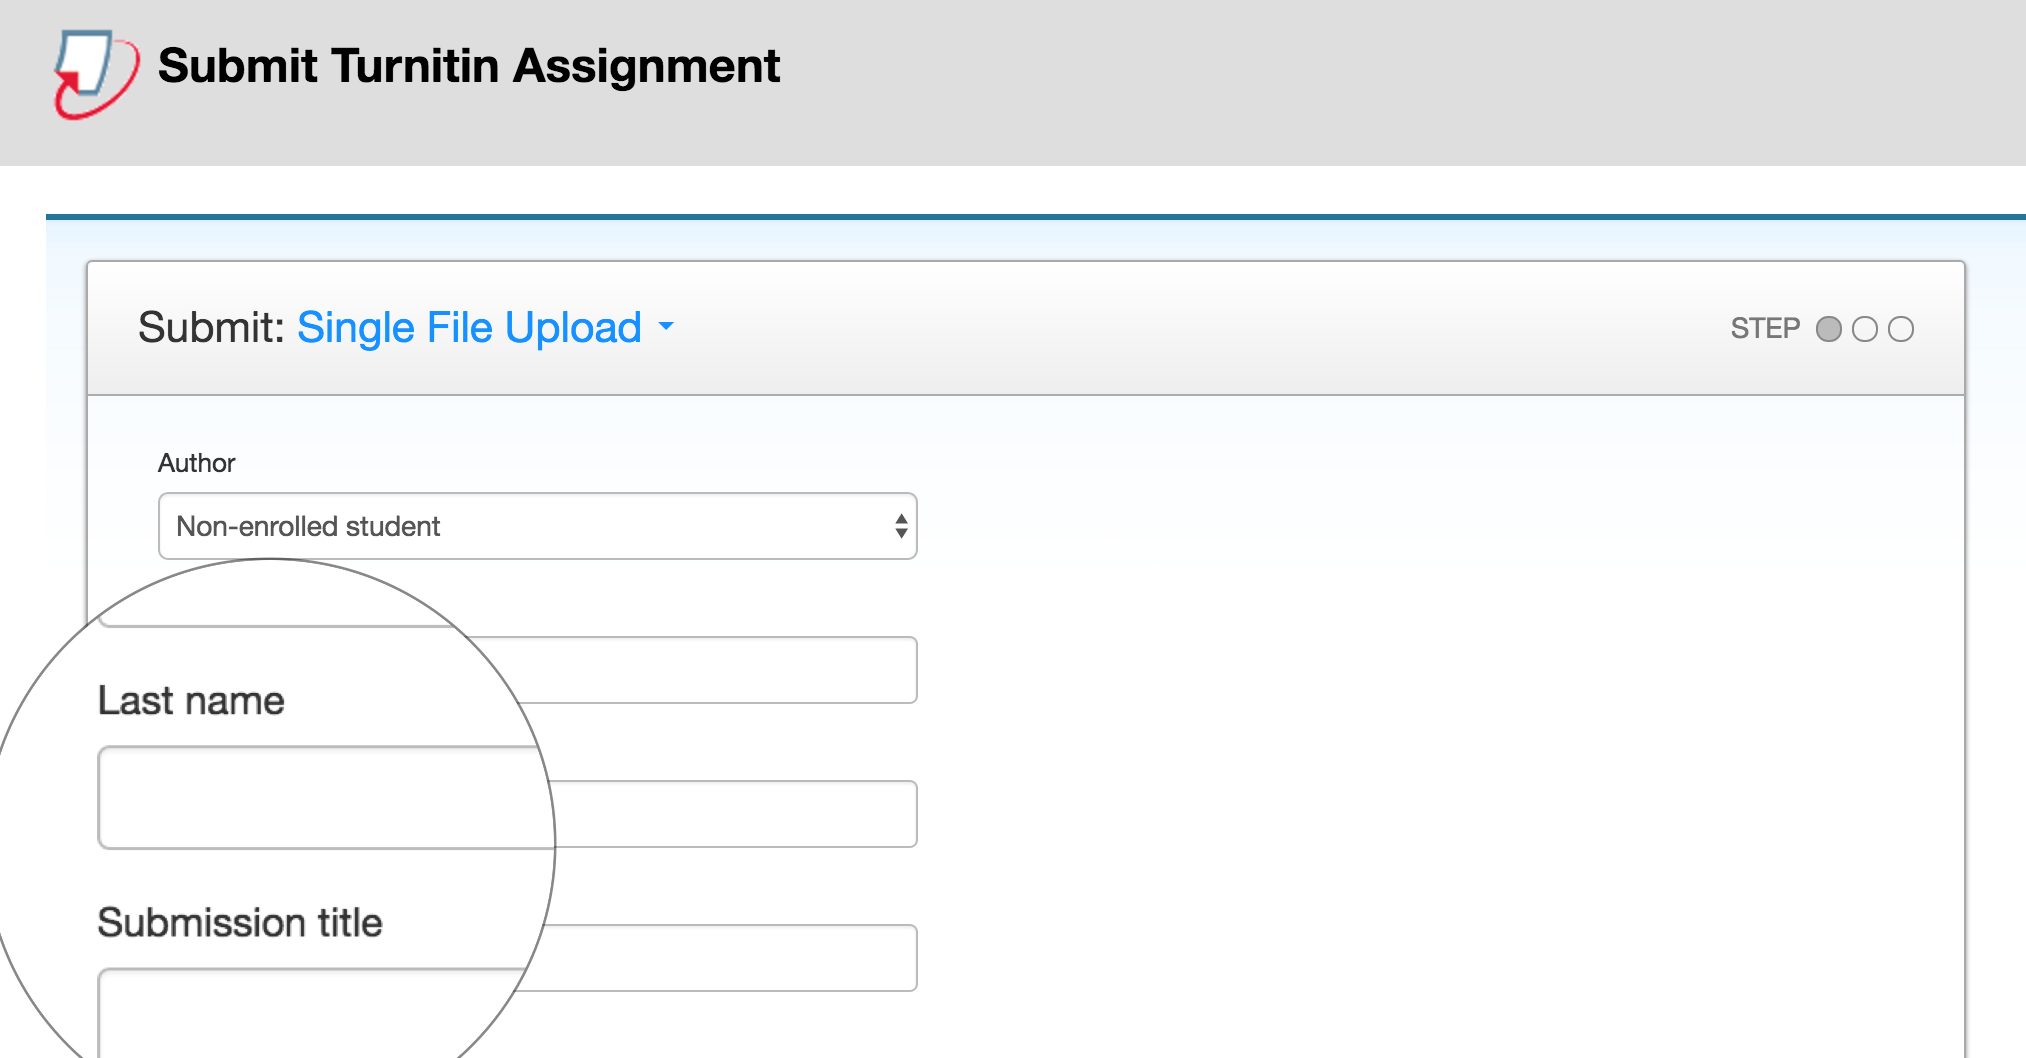
\includegraphics[height=4.5cm]{TurnitinSubmission.png}
\end{center}
\end{enumerate}







\newpage
\fbox{ {\bf Stats Report3 - Statistics in Research} }  {\tiny \bf  Submit this 1 Page Template.}

\begin{tabular}{|l|l|r|} \hline
{\bf Analysis} & {\bf Details} \hspace{11cm} & {\bf Mark} \\ \hline
Article & {\tiny Choose 1 of the given articles. List the title and author of the article and the journal reference.} &   \\
& & \\
& & \\ 
& & \\  \hline
Purpose & {\tiny What research question is being investigated?} & 1 \\
& & \\ 
& & \\ 
& & \\ 
& & \\ \hline
Summary & {\tiny How was statistics used in this article, and for what purpose?} & 2 \\
& & \\ 
& & \\ 
& & \\
& & \\ 
& & \\ 
& & \\ 
& & \\ 
& & \\ 
& & \\ 
& & \\ 
& & \\ 
& & \\ 
& & \\ 
& & \\ 
& & \\ 
& & \\ 
& & \\
& & \\ 
& & \\ 
& & \\
& & \\
& & \\\hline
Conclusion & {\tiny In your own words in 1 sentence, explain the conclusion of the article. Who would it be useful for?} & 1 \\
& & \\ 
& & \\
& & \\ 
& & \\ 
& & \\ 
& & \\ 
& & \\ 
& & \\
& & \\
& & \\ \hline
Research & {\tiny What is a question that could be investigated by further data analysis?} & 1 \\
&  &  \\ 
& & \\
& & \\ 
& & \\ \hline
Total & &  \\ 
& & /5 \\ \hline
\end{tabular}





\end{tutorial}
\end{document}

